\section{Menus}

\subsection{Menu principal}

\begin{figure}[h]
    \centering
    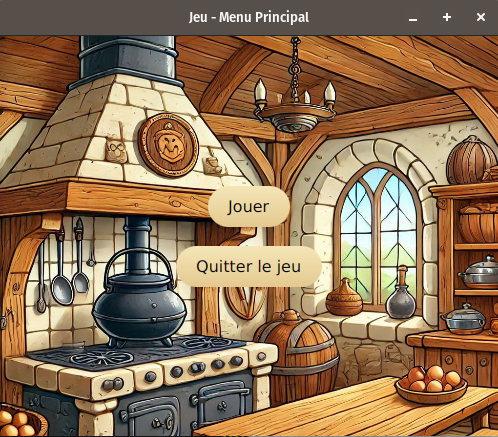
\includegraphics[width=18cm]{../Annexe/Screen/MenuPrincipale.png}
    \caption{Menu principal}
\end{figure}

Le menu principal est la première interface que vous rencontrerez en lançant l'application. Il permet d'accéder au jeu ou de quitter l'application.

\subsection{Gestion des Profils}

\begin{figure}[h]
    \centering
    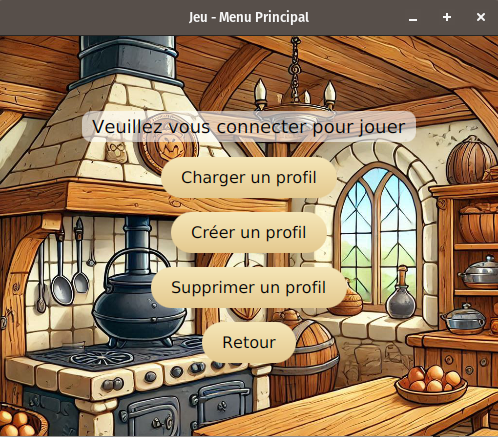
\includegraphics[width=15cm]{../Annexe/Screen/Profils.png}
    \caption{Gestion des profils}
\end{figure}

La gestion des profils permet aux utilisateurs de créer, supprimer, modifier, charger et consulter des profils.

\subsubsection{Création d'un Profil}

Pour créer un nouveau profil utilisateur :

\begin{itemize}
  \item Accédez à la section de gestion des profils.
  \item Sélectionnez l'option \og Créer un profil \fg.
  \item Saisissez un nom d'utilisateur unique.
  \item Une fois validé, le nouveau profil sera créé et disponible.
\end{itemize}

\subsubsection{Suppression d'un Profil}

Pour supprimer un profil utilisateur :

\begin{itemize}
  \item Accédez à la section de gestion des profils.
  \item Sélectionnez \og Supprimer un profil \fg.
  \item Entrez le nom du profil à supprimer.
  \item Confirmez la suppression.
\end{itemize}

\subsubsection{Chargement d'un Profil}

Pour charger un profil utilisateur :

\begin{itemize}
  \item Accédez à la gestion des profils.
  \item Sélectionnez \og Charger un profil \fg.
  \item Choisissez un profil existant.
  \item Le profil est activé pour la session.
\end{itemize}

\subsection{Sélection des Difficultés}

\begin{figure}[h]
    \centering
    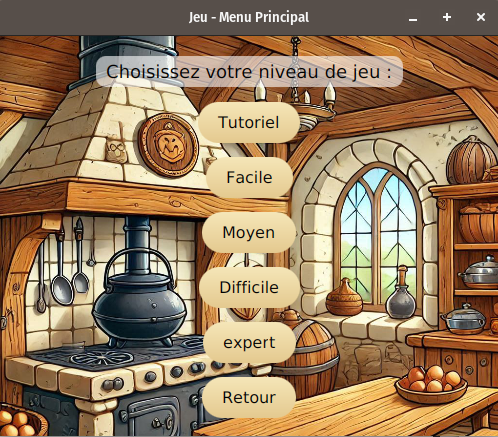
\includegraphics[width=15cm]{../Annexe/Screen/difficulte.png}
    \caption{Sélection des difficultés}
\end{figure}

Dès qu'un profil est sélectionné, l'utilisateur peut choisir un niveau de difficulté :

\begin{itemize}
    \item \textbf{Tutoriel} : Explication de l'interface et des règles.
    \item \textbf{Facile} : Convient aux débutants.
    \item \textbf{Moyen} : Idéal pour tester des stratégies.
    \item \textbf{Difficile} : Pour ceux qui aiment les défis.
    \item \textbf{Expert} : Un niveau extrême pour les joueurs expérimentés.
\end{itemize}
\newpage
\subsection{Fenêtre de Jeu}

\begin{figure}[h]
    \centering
    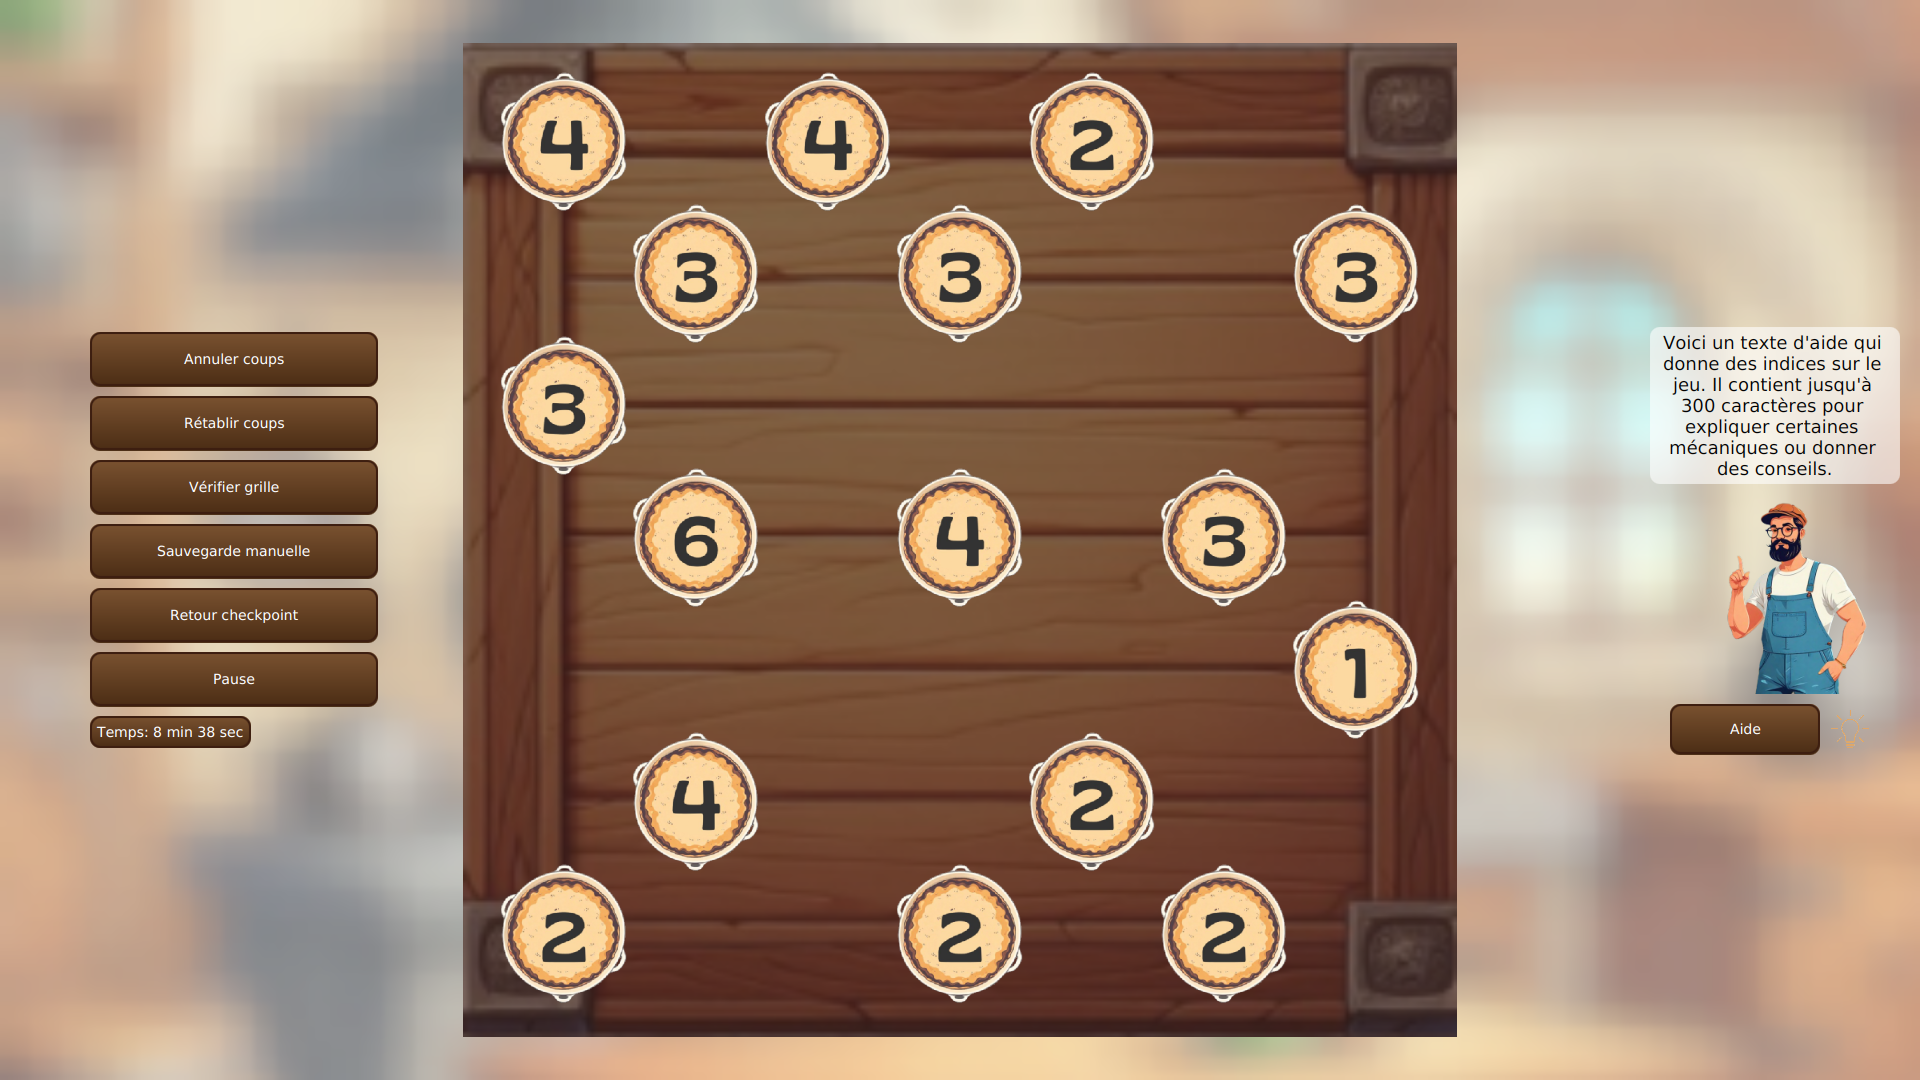
\includegraphics[width=15cm]{../Annexe/Screen/FenetreJeu.png}
    \caption{Fenêtre de jeu}
\end{figure}

La fenêtre de jeu représente la grille de Hashi et permet de jouer tout en vérifiant les réponses en temps réel.

\begin{figure}[h]
    \centering
    \begin{minipage}{0.4\textwidth}
        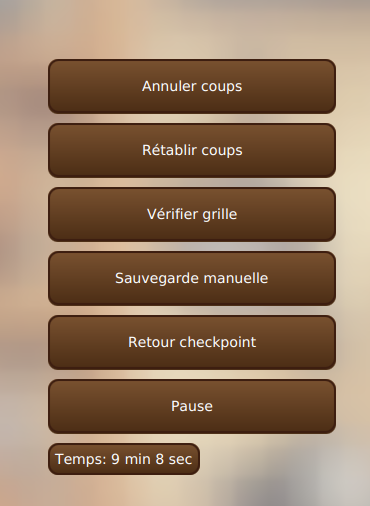
\includegraphics[width=6cm]{../Annexe/Screen/MenuD.png}
        \caption{Menu latéral}
    \end{minipage}%
    \hfill
    \begin{minipage}{0.55\textwidth}
        \begin{itemize}
            \item \textbf{Annuler coups} : Annule tous les coups réalisés.
            \item \textbf{Rétablir coups} : Rétablit un coup annulé (si aucun autre coup n'a été joué entre-temps).
            \item \textbf{Vérifier grille} : Revenir au dernier état valide.
            \item \textbf{Sauvegarde manuelle} : Enregistre un état de la grille.
            \item \textbf{Retour checkpoint} : Revenir à une sauvegarde précédente.
            \item \textbf{Pause} : Accède au menu pause et arrête le temps.
            \item \textbf{Temps} : Affiche le temps de jeu (avec pénalités en cas d'utilisation d'aides).
        \end{itemize}
    \end{minipage}
\end{figure}
\\
\pagebreak
Au centre la fenêtre, nous avons la grille de jeu avec les iles représenter par des Hachi Parmentier et les liens par des fils de fromage fondu.\\
Le survol d'un lien possible met en évidence son activation. Les iles prennent plusieurs couleurs en fonction de leurs états:
\begin{figure}[h]
    \centering
    \begin{minipage}{0.4\textwidth}
        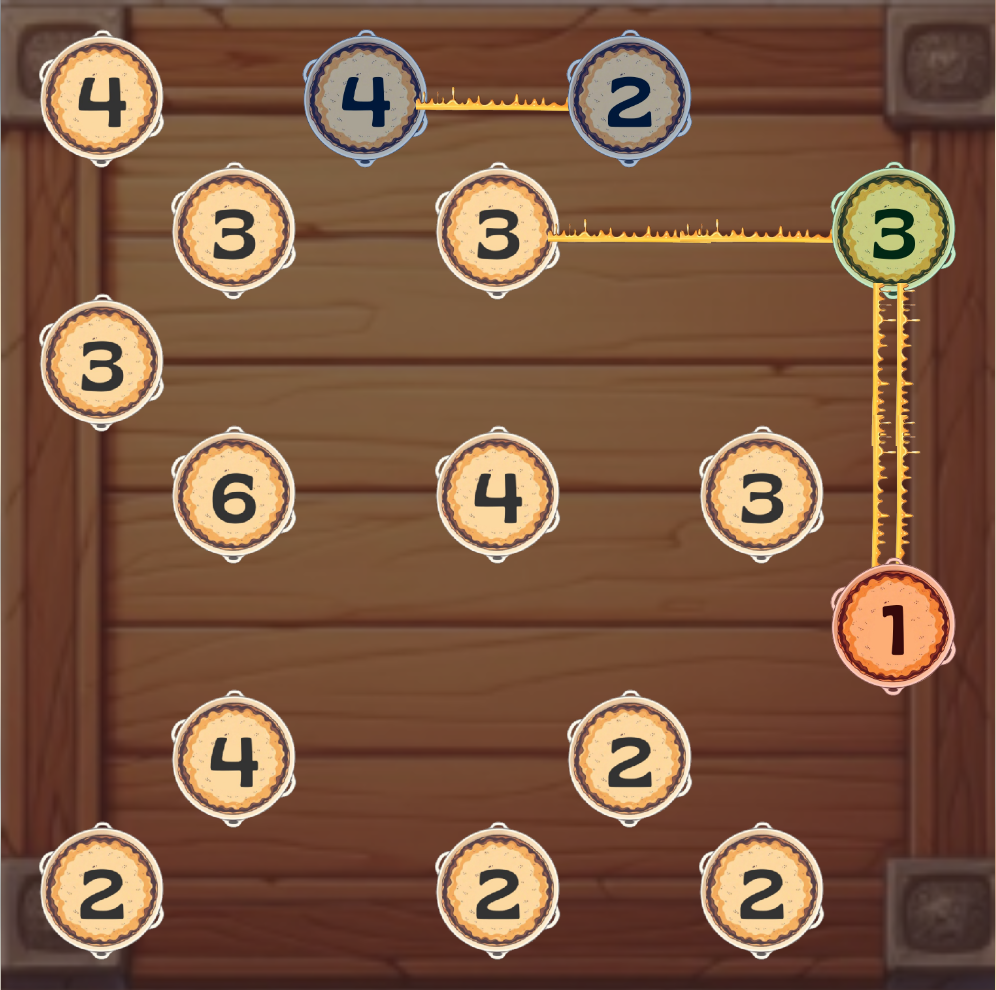
\includegraphics[width=6cm]{../Annexe/Screen/Grille.png}
        \caption{Grille de jeu}
    \end{minipage}%
    \hfill
    \begin{minipage}{0.55\textwidth}
        
        \begin{itemize}
            \item \textbf{Rouge} : Trop de liens.
            \item \textbf{Vert} : Nombre de liens correct.
            \item \textbf{Bleu} : Île activée et réseau affiché.
            \item \textbf{Aucune couleur} : Île non connectée ou liens insuffisants.
        \end{itemize}
    \end{minipage}
\end{figure}
\\
Sur la droite, une option permet de demander de l'aide en fonction de l'état de la grille. Les aides fournis dépendent du niveau d'aide choisis dans les options.
\begin{figure}[h]
    \centering
    \begin{minipage}{0.4\textwidth}
        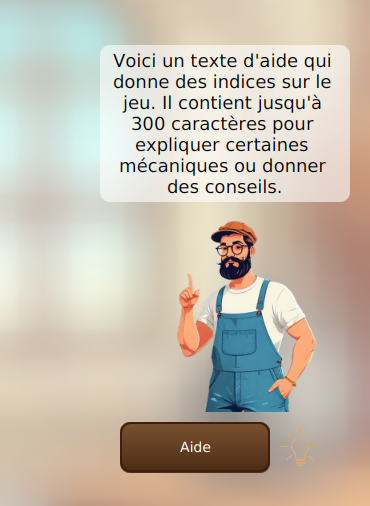
\includegraphics[width=6cm]{../Annexe/Screen/Aide.png}
        \caption{Menu d'aide}
    \end{minipage}%
    \hfill
    \begin{minipage}{0.55\textwidth}
    \begin{itemize}
        \item \textbf{Facile :}  Une aide légère, qui convient aux personnes assez avancée
        \item \textbf{Normal :} Permet d'acceder aux aides facile et fournit aussi une aide plus précise
        \item \textbf{Difficile :} Permet d'acceder aux aides facile et normal et fournit une aide plus poussée pour le joueur.
    \end{itemize}
    \end{minipage}
\end{figure}

\\
\pagebreak
\subsection{Pause}
Lorsque le jeu est en pause, le temps est suspendu. Ce menu est accessible à tout moment et propose :

\begin{figure}[h]
    \centering
    \begin{minipage}{0.4\textwidth}
        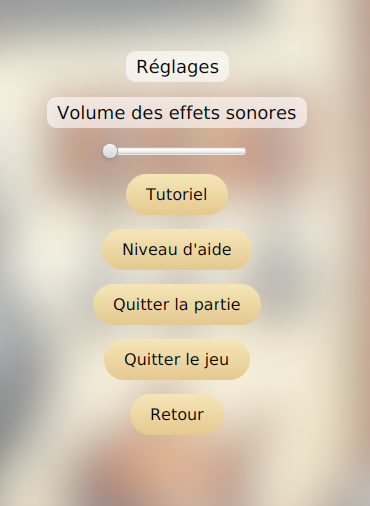
\includegraphics[width=7cm]{../Annexe/Screen/Pause.png}
        \caption{Menu pause}
    \end{minipage}%
    \hfill
    \begin{minipage}{0.55\textwidth}
        \begin{itemize}
            \item \textbf{Volume des effets sonores} : Ajuste le volume (par défaut 50 \%).
            \item \textbf{Tutoriel} : Consulte les règles et spécificités du jeu.
            \item \textbf{Niveau d'aide} : Choisit le niveau d'assistance.
            \item \textbf{Quitter la partie} : Retour au menu principal.
            \item \textbf{Quitter le jeu} : Ferme l'application.
            \item \textbf{Retour} : Reprend la partie.
        \end{itemize}
    \end{minipage}
\end{figure}
